\chapter{Appendix F: Extra Plots and Figured}
\label{AppendixF}

\section{Extra SOBOL Analyses}
\label{sec:AppendixF:extra_SOBOL_analyses}

\begin{figure}
    \centering
    \begin{subfigure}{0.49\linewidth}
        \centering
        \captionsetup{width=1\linewidth}
        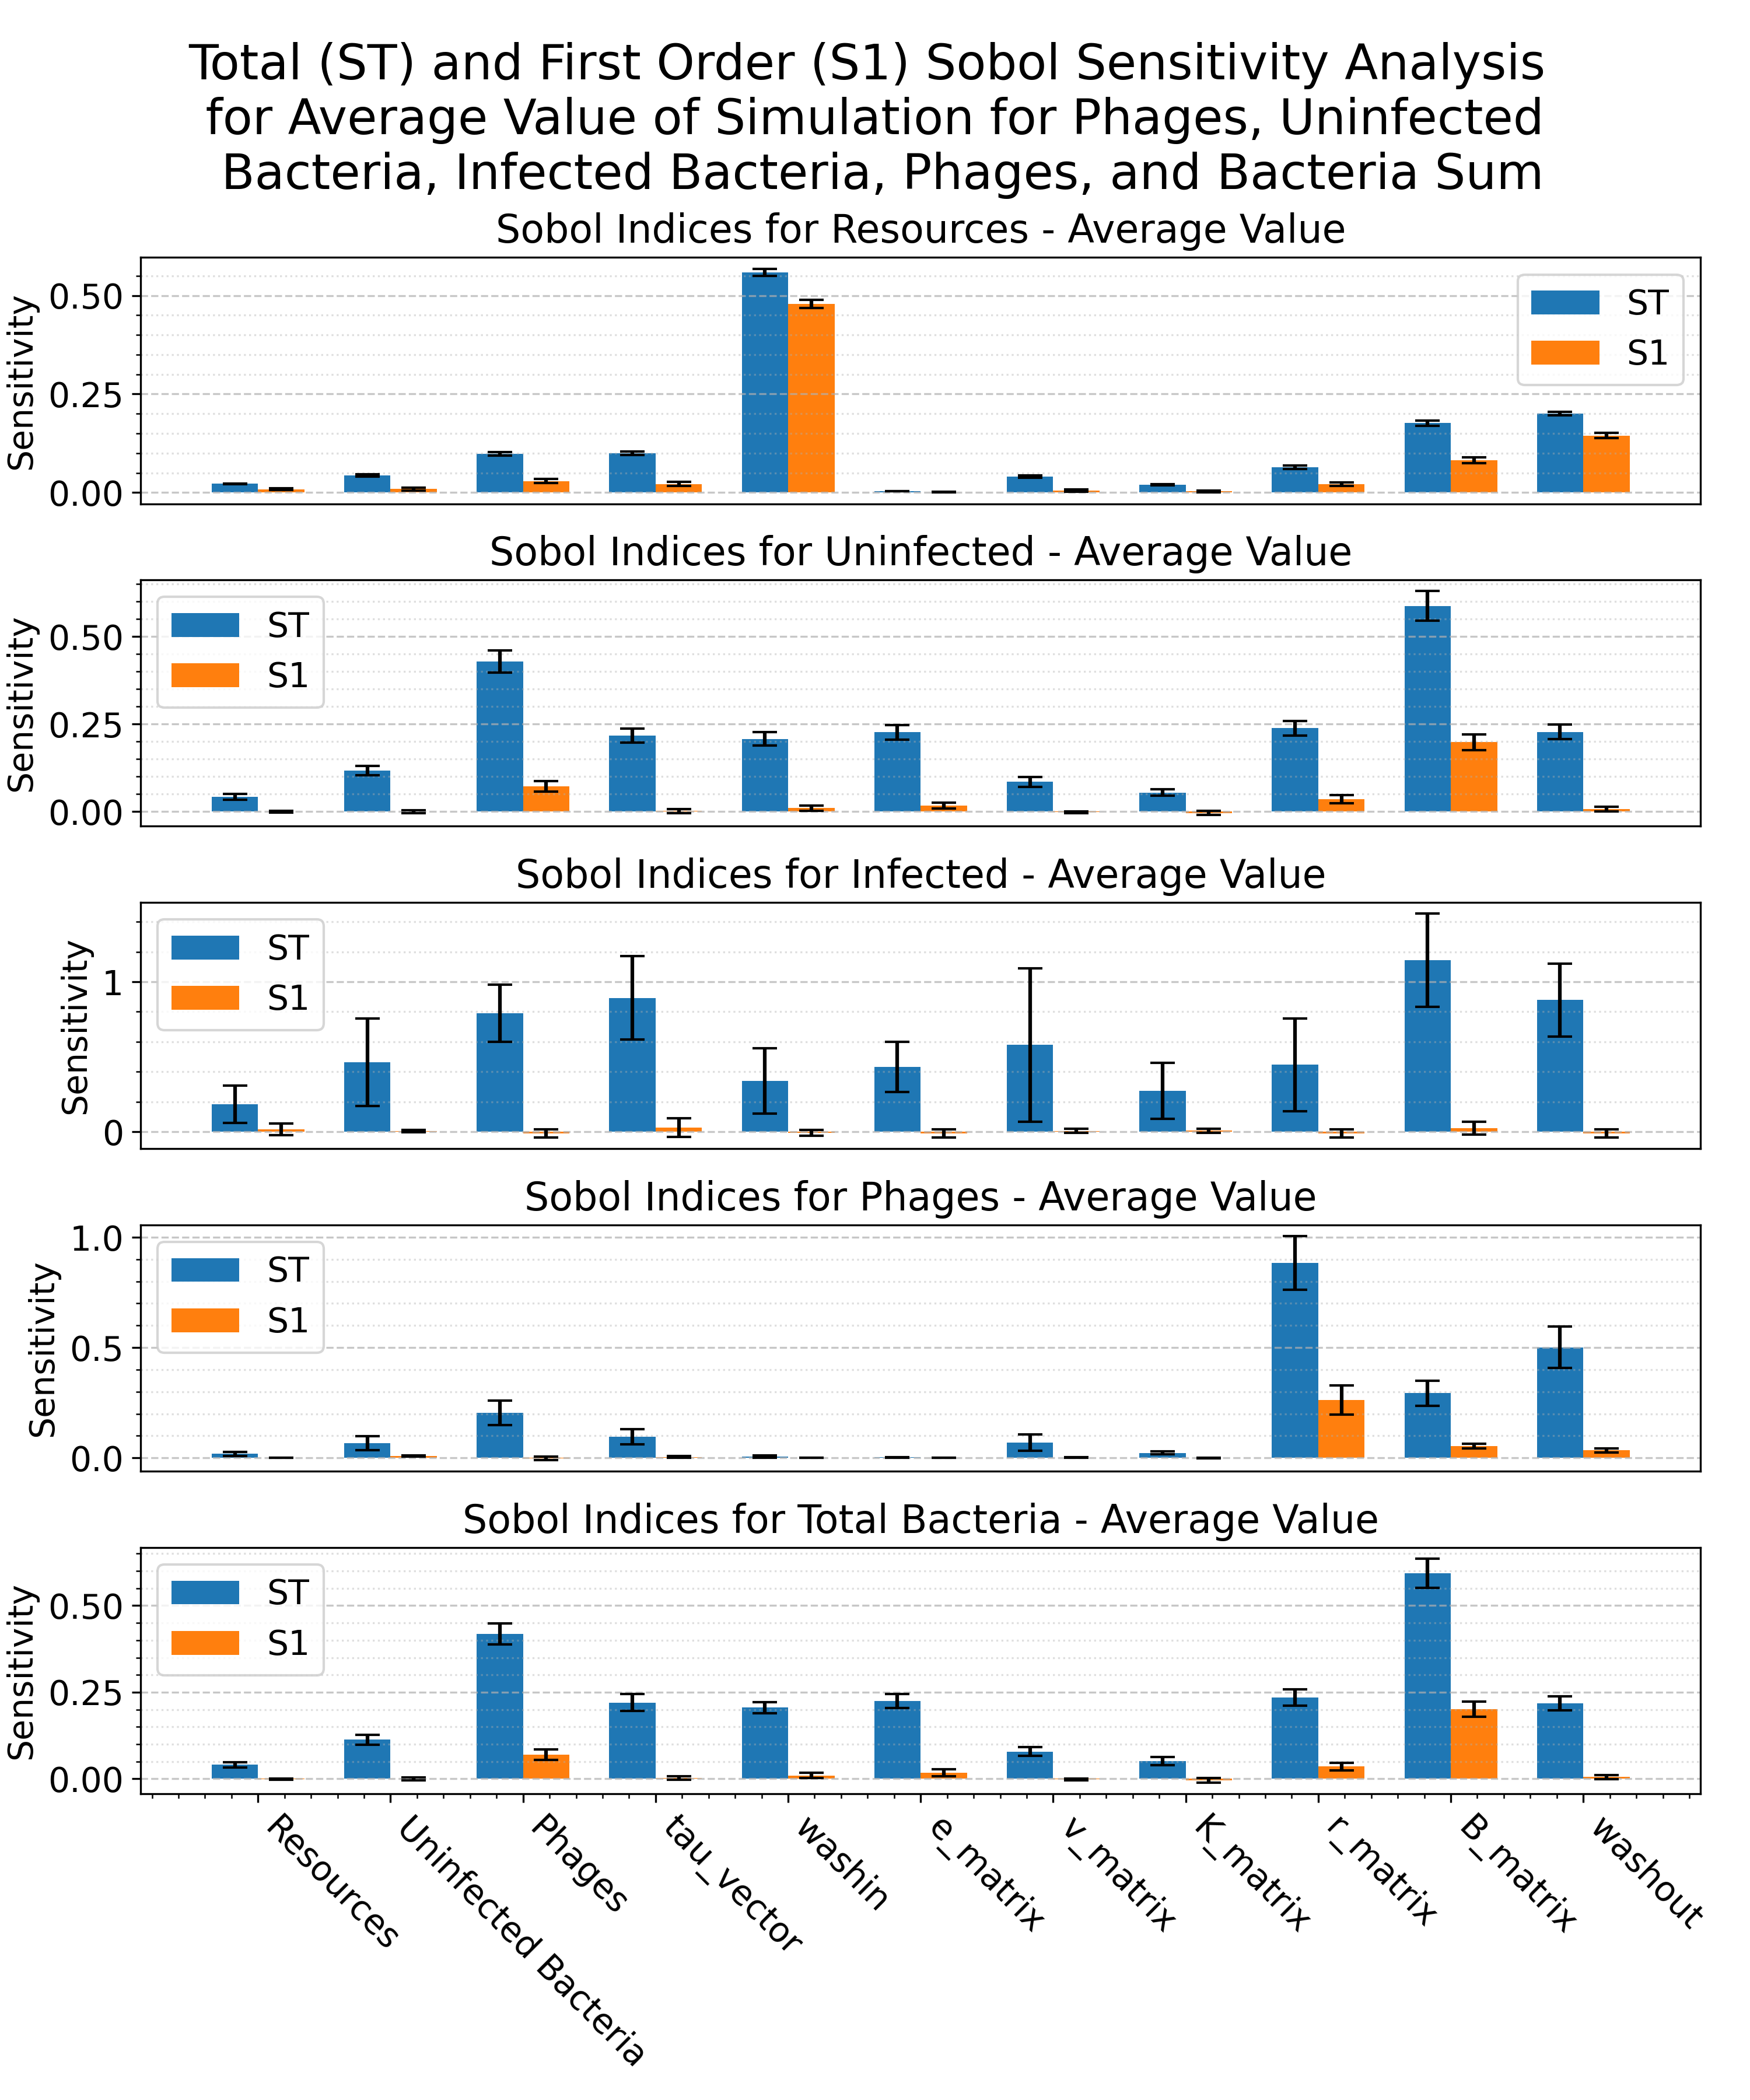
\includegraphics[width=\linewidth]{Plots/Created/SOBOL_analysis_1748084143_Average.png}
        \caption{
            The $ST$ and $S1$ sensitivity for the average Resource, Uninfected, Infected, Phage, and Total Bacteria population. 
        }
        \label{fig:created:SOBOL_average_extra}
    \end{subfigure}
    \hfill
    \begin{subfigure}{0.49\linewidth}
        \centering
        \captionsetup{width=1\linewidth}
        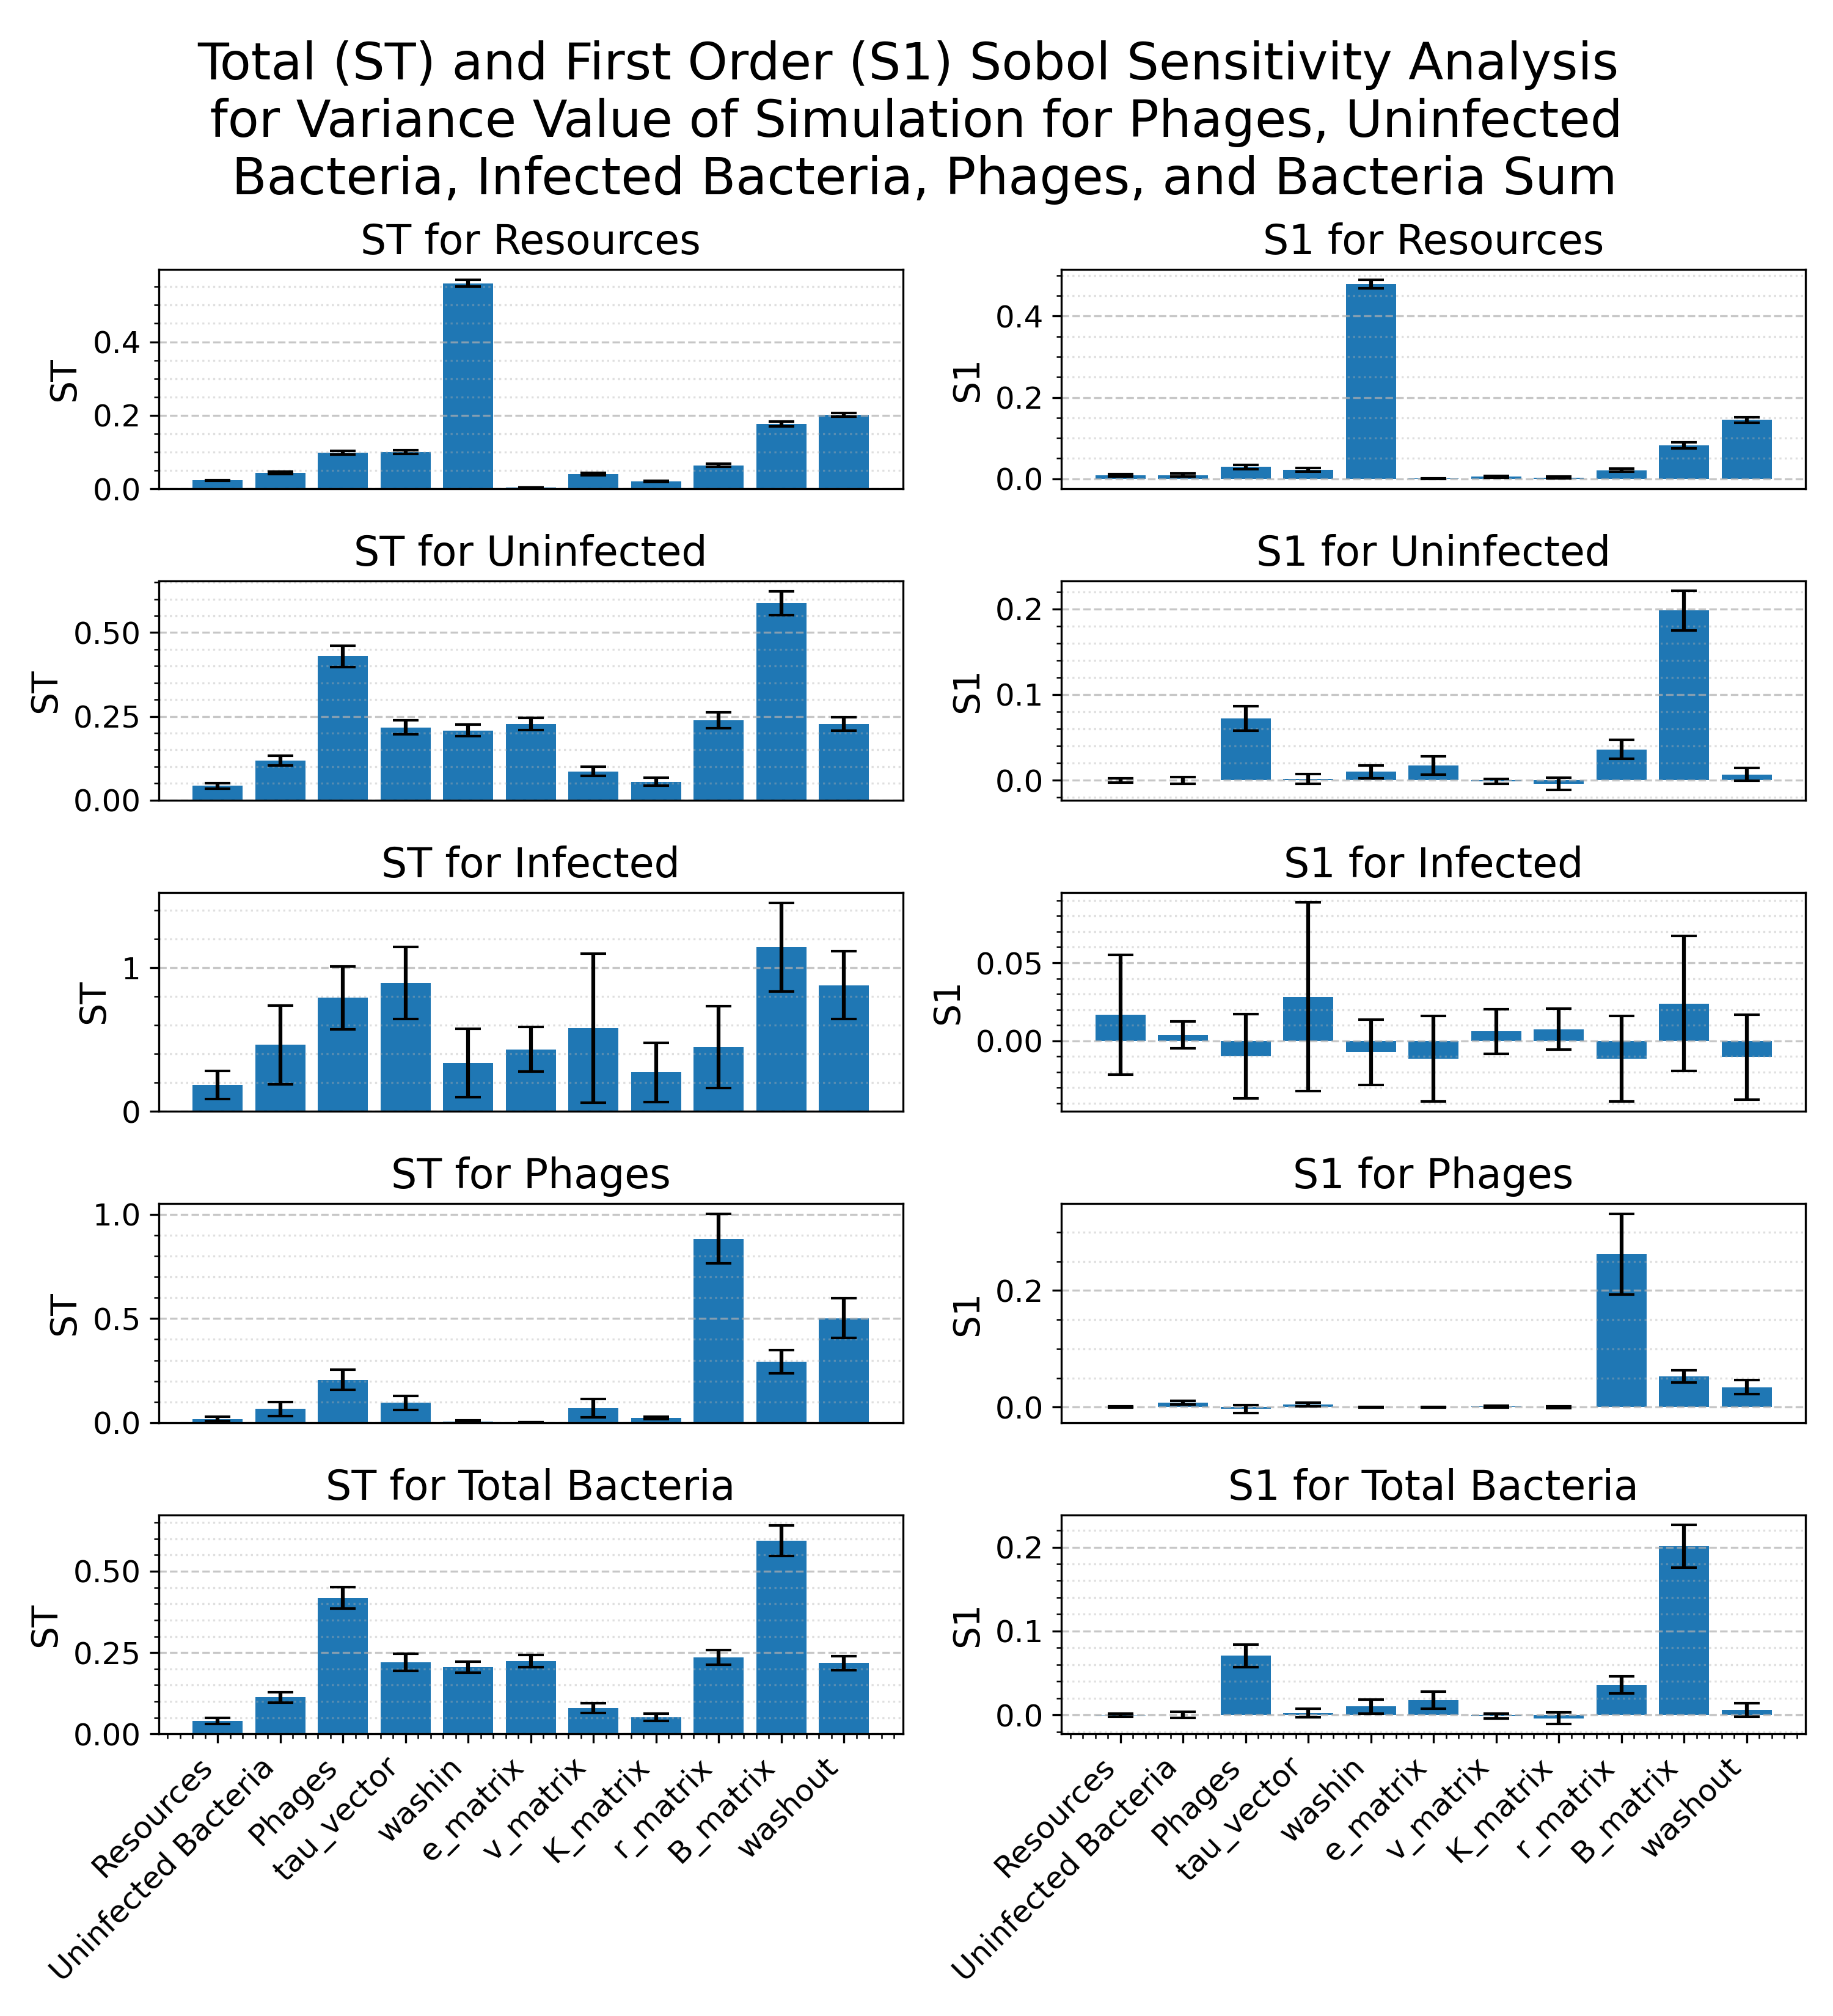
\includegraphics[width=\linewidth]{Plots/Created/SOBOL_analysis_1748084143_Variance.png}
        \caption{
            The $ST$ and $S1$ sensitivity for the variance of the Resource, Uninfected, Infected, Phage, and Total Bacteria population. 
        }
        \label{fig:created:SOBOL_variance_extra}
    \end{subfigure}
    \caption{
        SOBOL analyses for the average, peak, and peak time. 
        The data was saved from the dashboard and plotted using Matplotlib. 
        The values used for this SOBOL test can be found in \Cref{tab:appendixE:SOBOL_analysis_values}. 
        The same data used in \Cref{fig:created:SOBOL_analyses} was used for \Cref{fig:created:SOBOL_average_extra} and \Cref{fig:created:SOBOL_variance_extra}. 
    }
    \label{fig:created:SOBOL_extra}
\end{figure}


\subsection{SOBOL Analysis Without Washin and Washout}
\begin{figure}
    \centering
    \begin{subfigure}{0.32\linewidth}
        \centering
        \captionsetup{width=1\linewidth}
        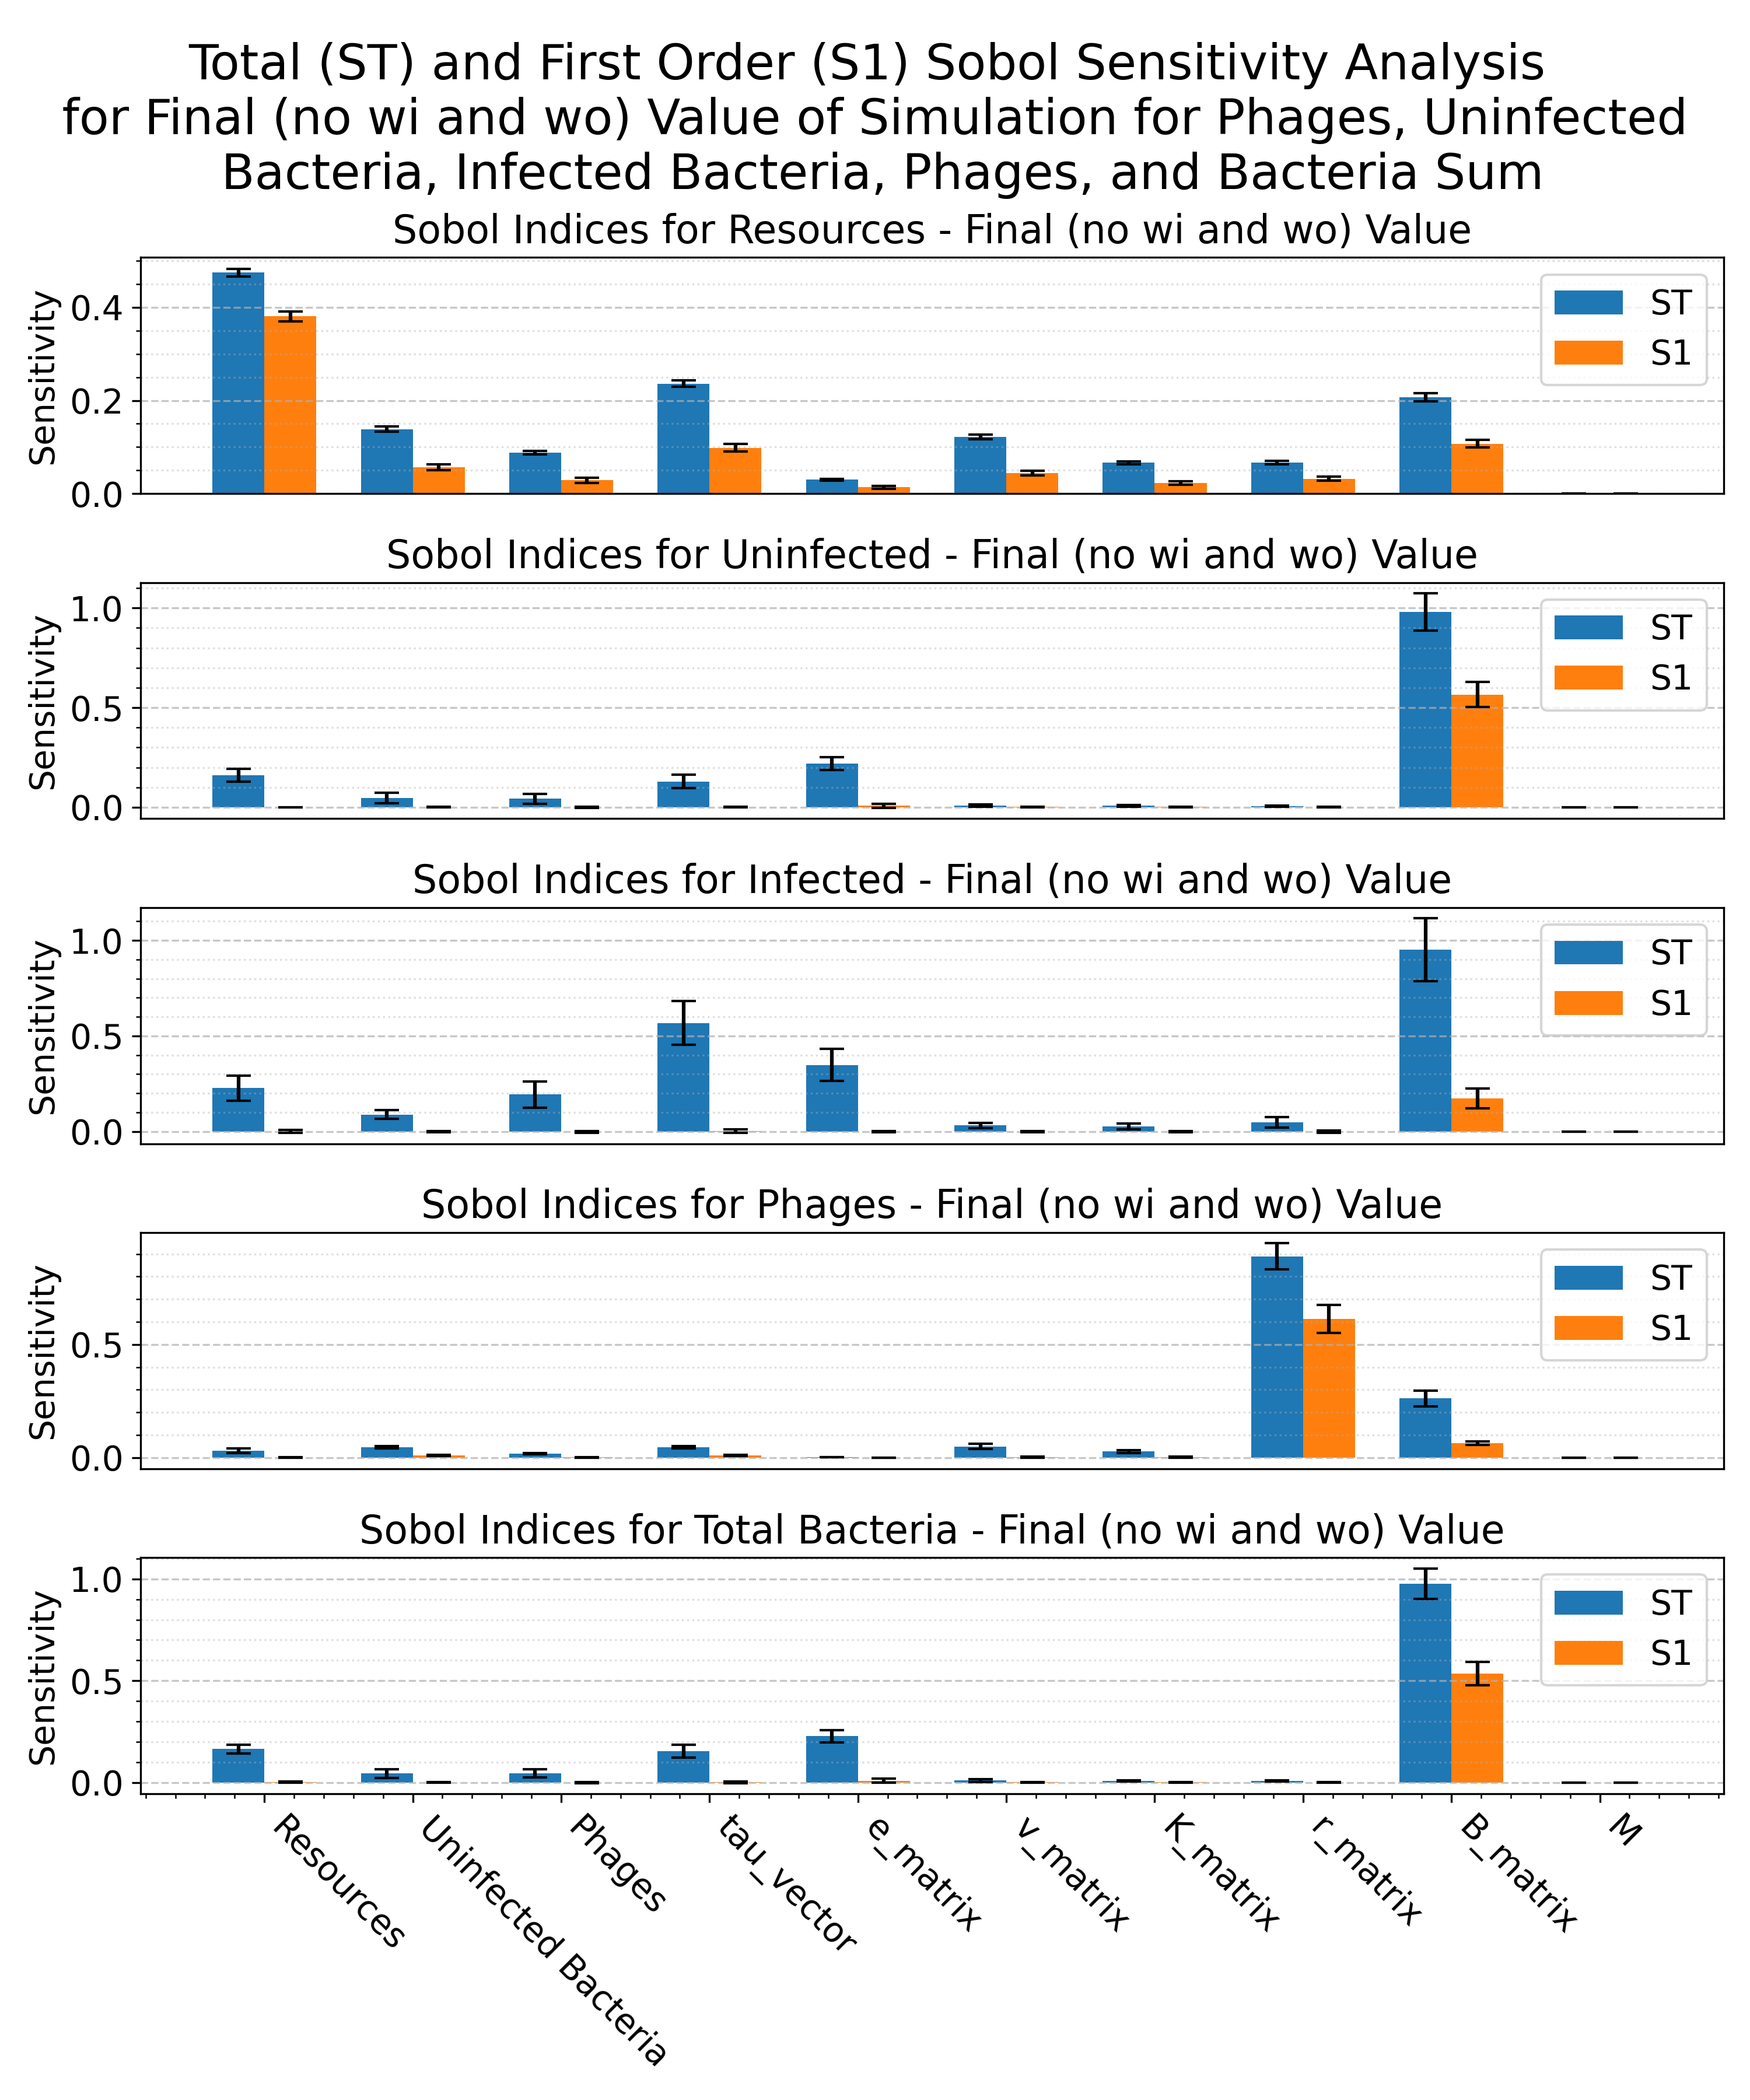
\includegraphics[width=\linewidth]{Plots/Created/SOBOL_analysis_1748084143_Final_(no_wi_and_wo).png}
        \caption{
            Final value, no washin and washout. 
        }
        \label{fig:created:SOBOL_final_no_wi_wo_extra}
    \end{subfigure}
    \hfill
    \begin{subfigure}{0.32\linewidth}
        \centering
        \captionsetup{width=1\linewidth}
        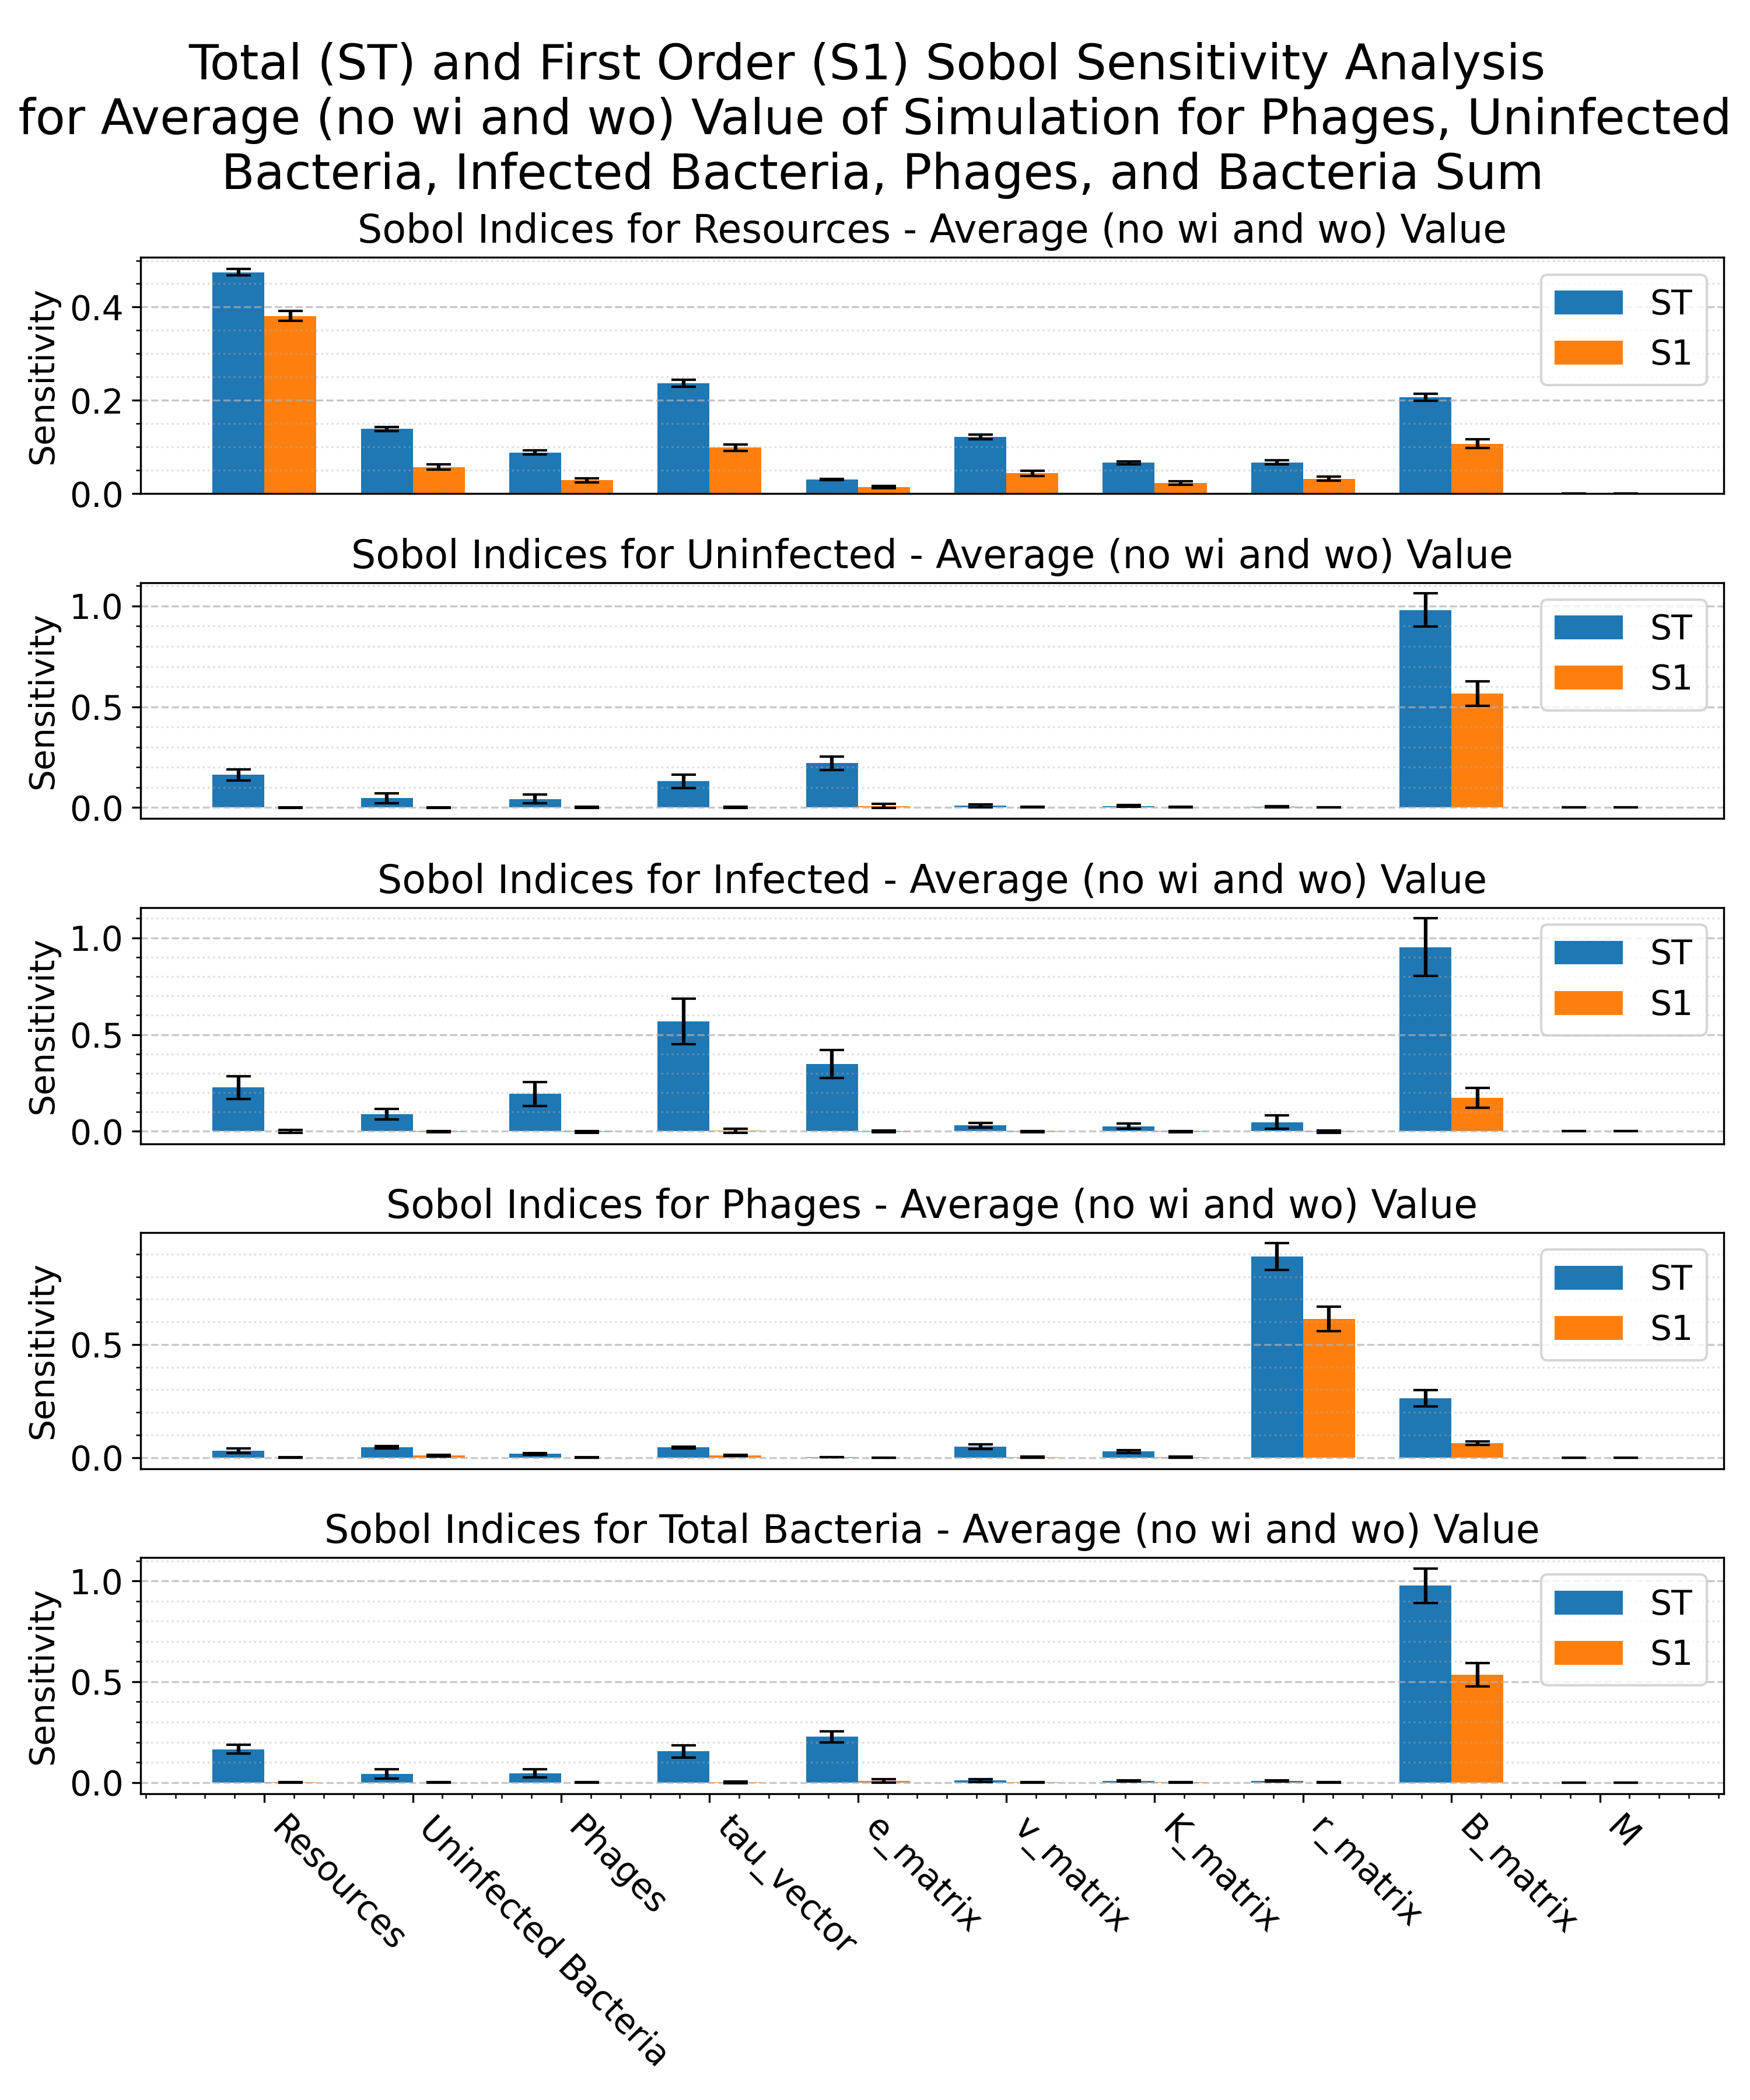
\includegraphics[width=\linewidth]{Plots/Created/SOBOL_analysis_1748084143_Average_(no_wi_and_wo).png}
        \caption{
            Average value, no washin and washout. 
        }
        \label{fig:created:SOBOL_average_no_wi_wo_extra}
    \end{subfigure}
    \hfill
    \begin{subfigure}{0.32\linewidth}
        \centering
        \captionsetup{width=1\linewidth}
        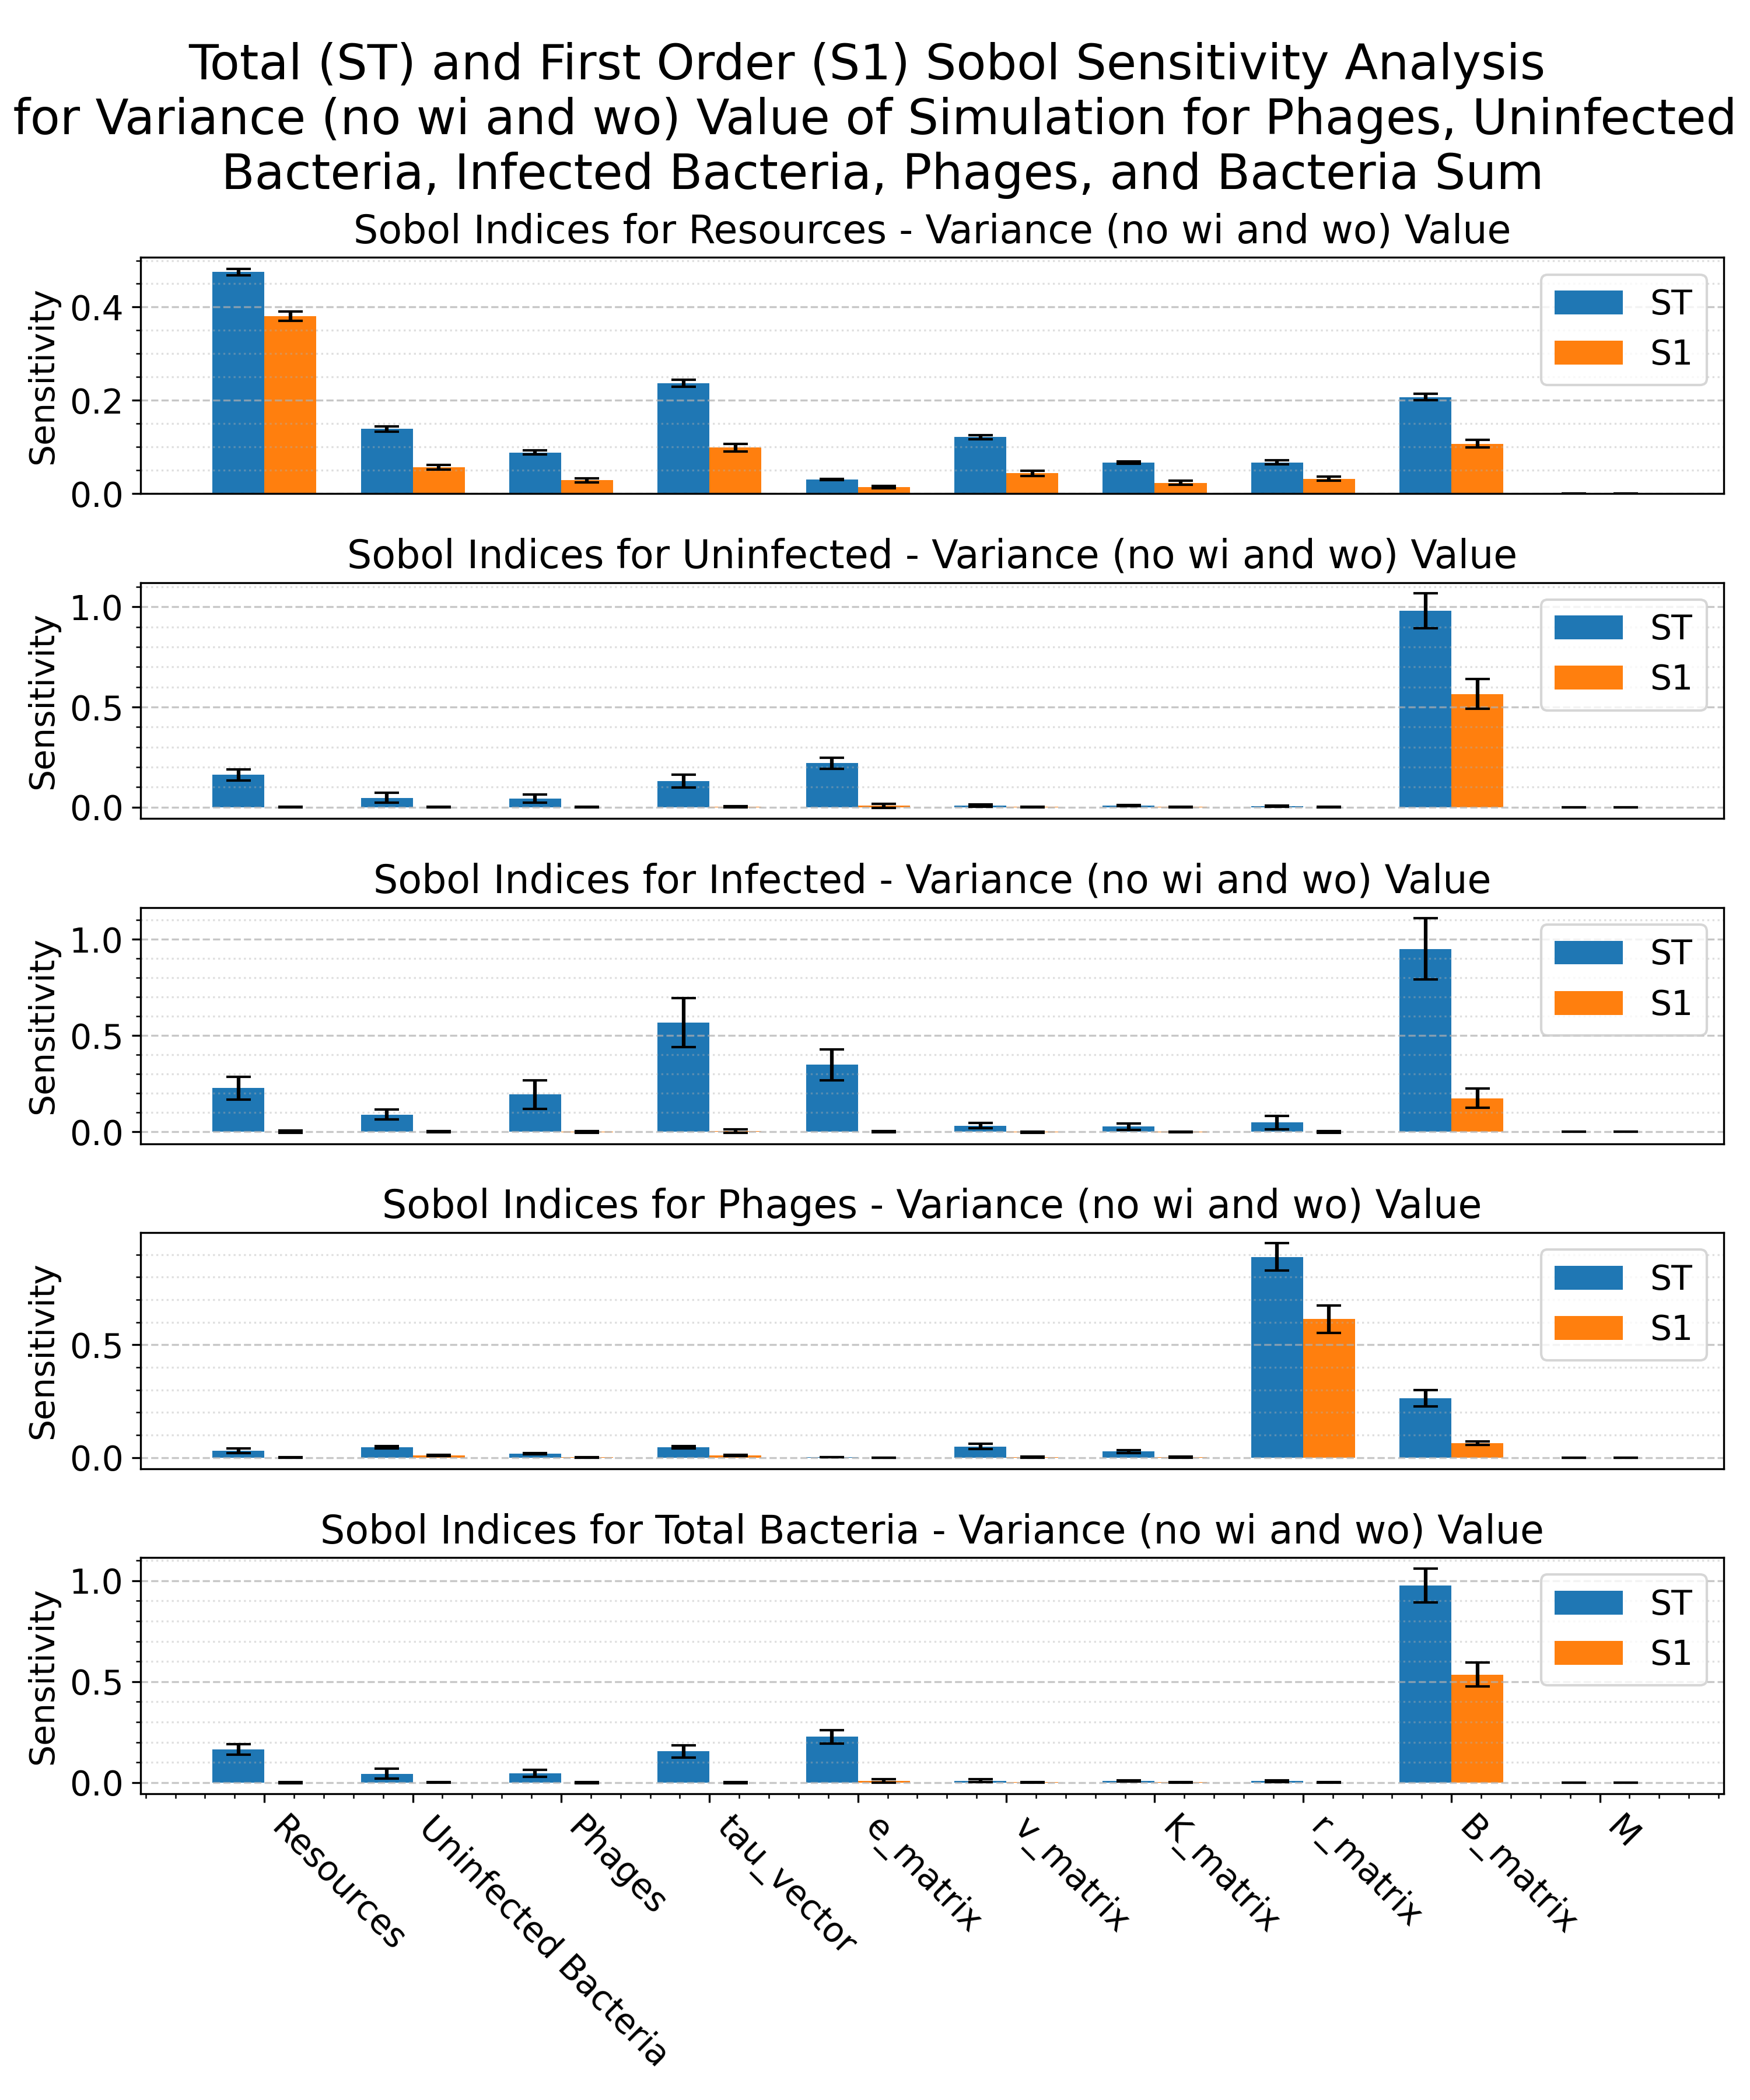
\includegraphics[width=\linewidth]{Plots/Created/SOBOL_analysis_1748084143_Variance_(no_wi_and_wo).png}
        \caption{
            Variance of population value, no washin and washout. 
        }
        \label{fig:created:SOBOL_variance_no_wi_wo_extra}
    \end{subfigure}
    \hfill
    \begin{subfigure}{0.32\linewidth}
        \centering
        \captionsetup{width=1\linewidth}
        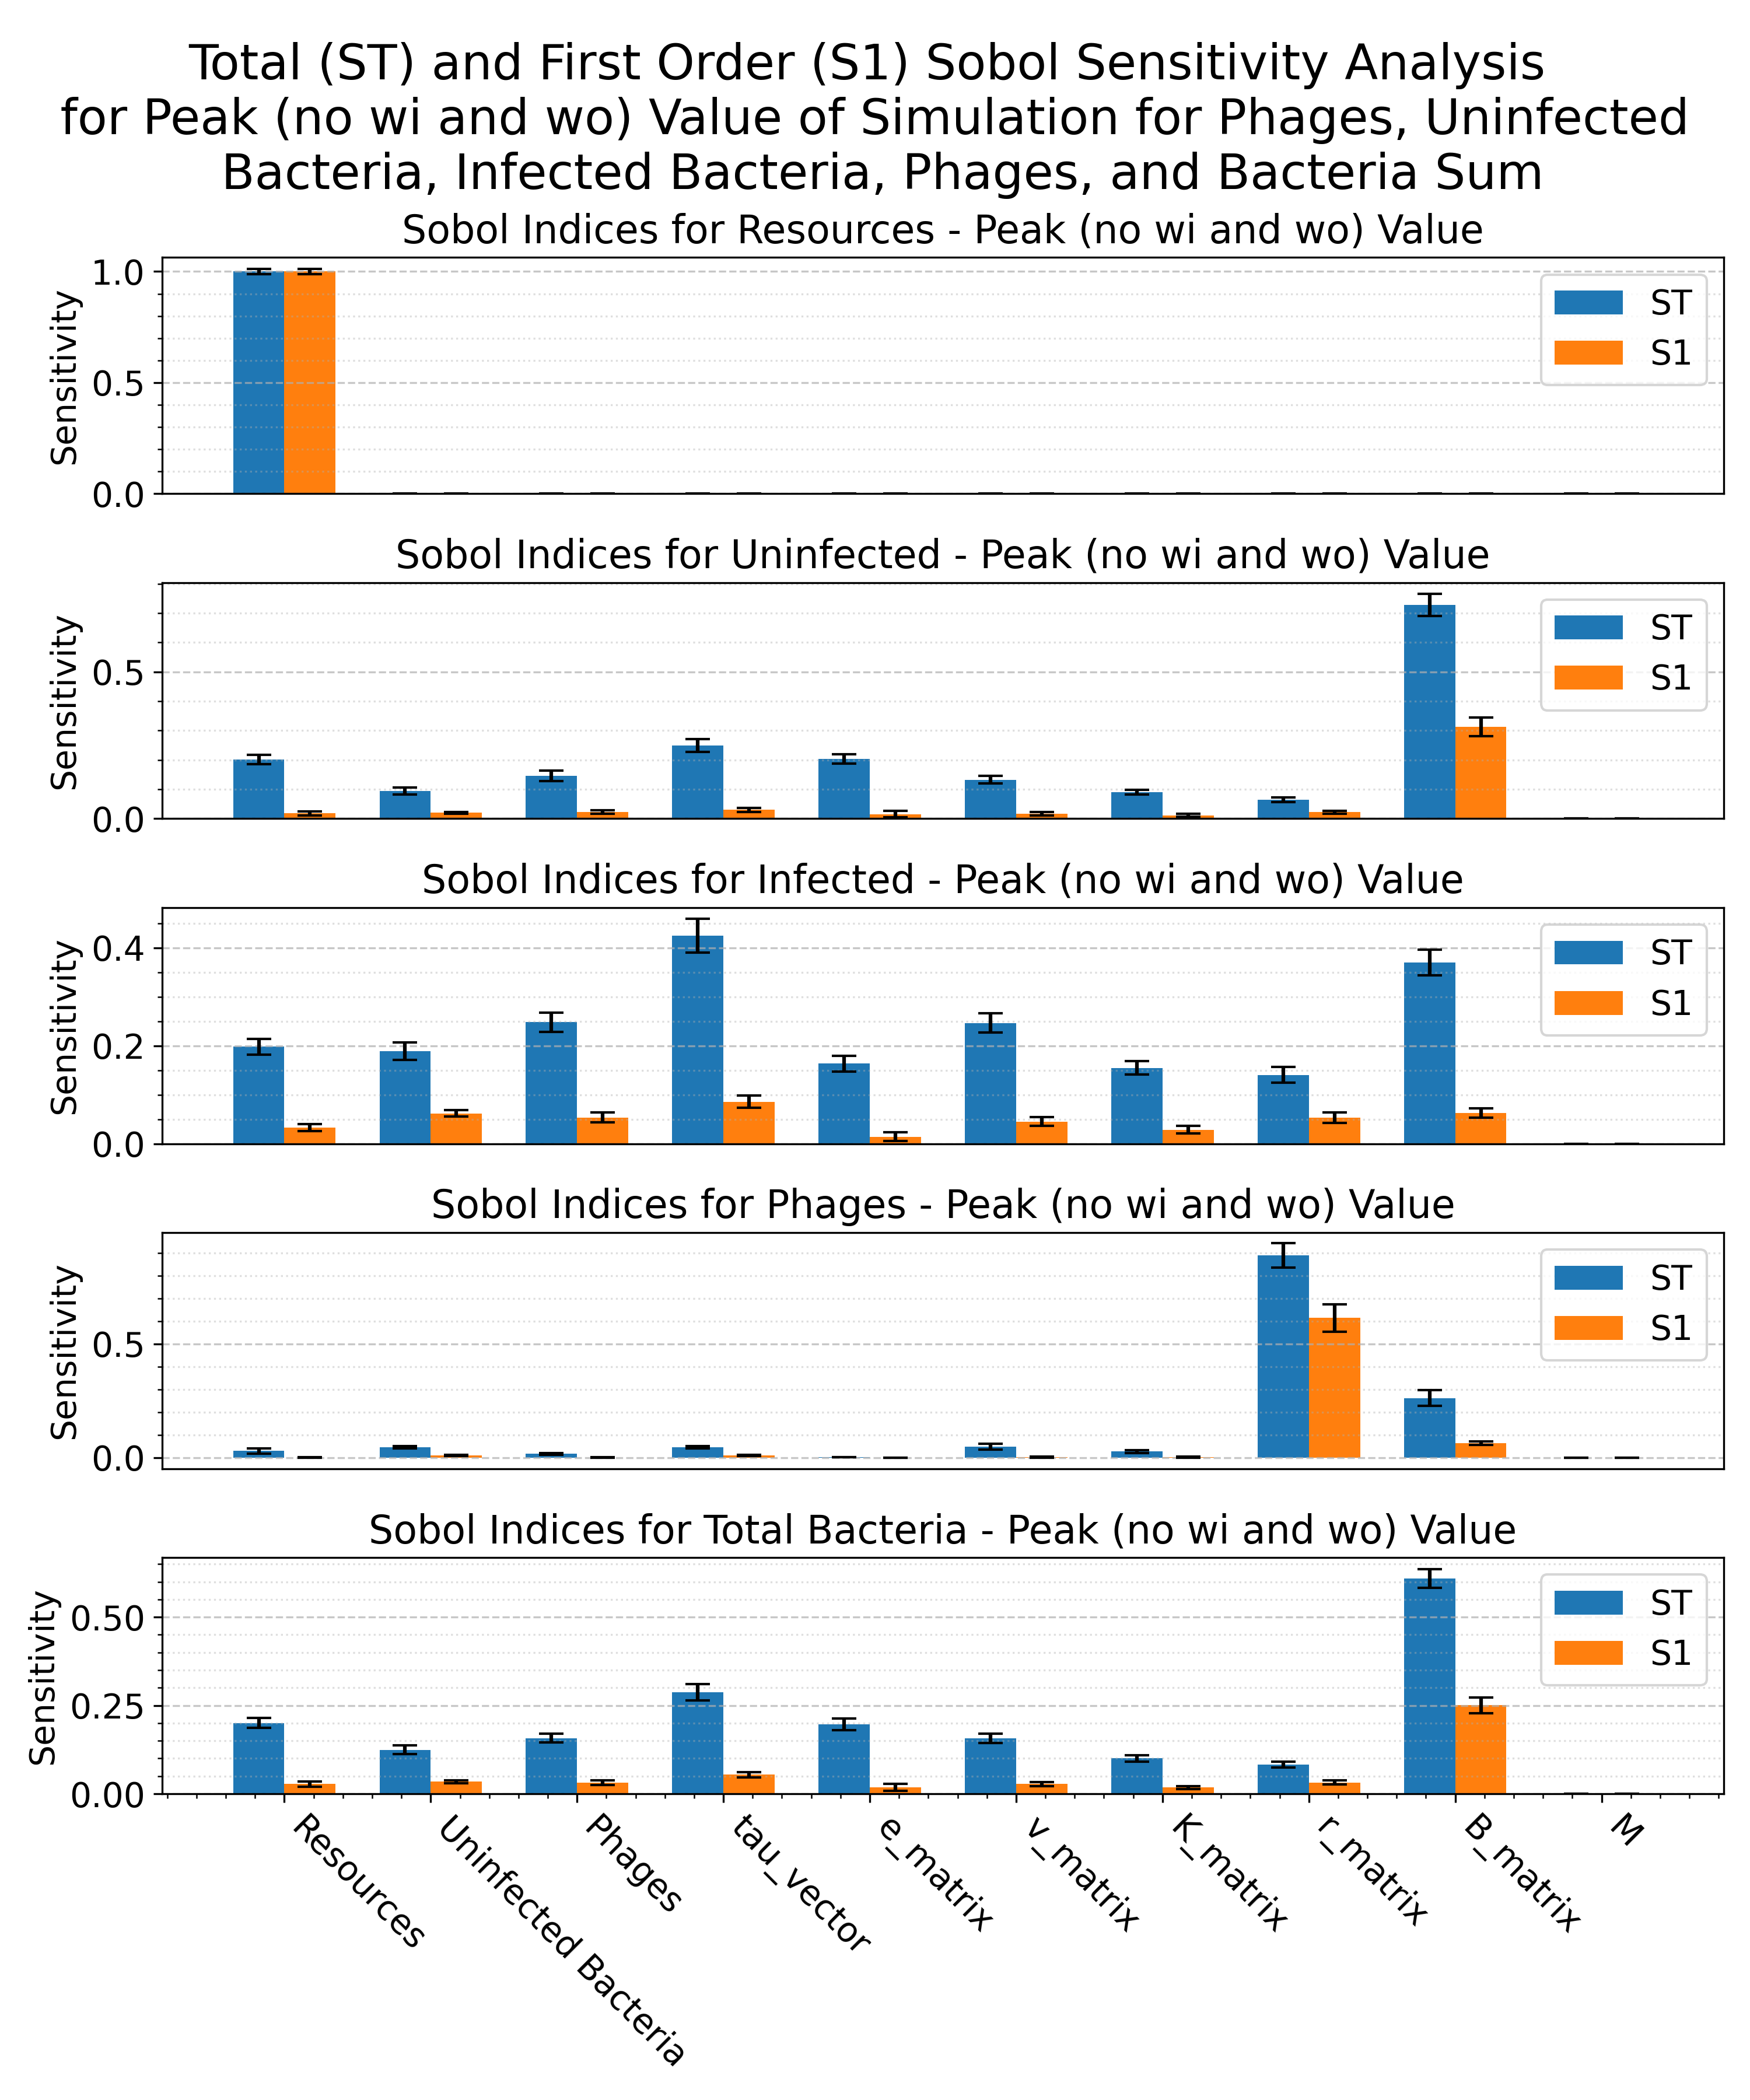
\includegraphics[width=\linewidth]{Plots/Created/SOBOL_analysis_1748084143_Peak_(no_wi_and_wo).png}
        \caption{
            Peak population value, no washin and washout. 
        }
        \label{fig:created:SOBOL_peak_no_wi_wo_extra}
    \end{subfigure}
    \hfill
    \begin{subfigure}{0.32\linewidth}
        \centering
        \captionsetup{width=1\linewidth}
        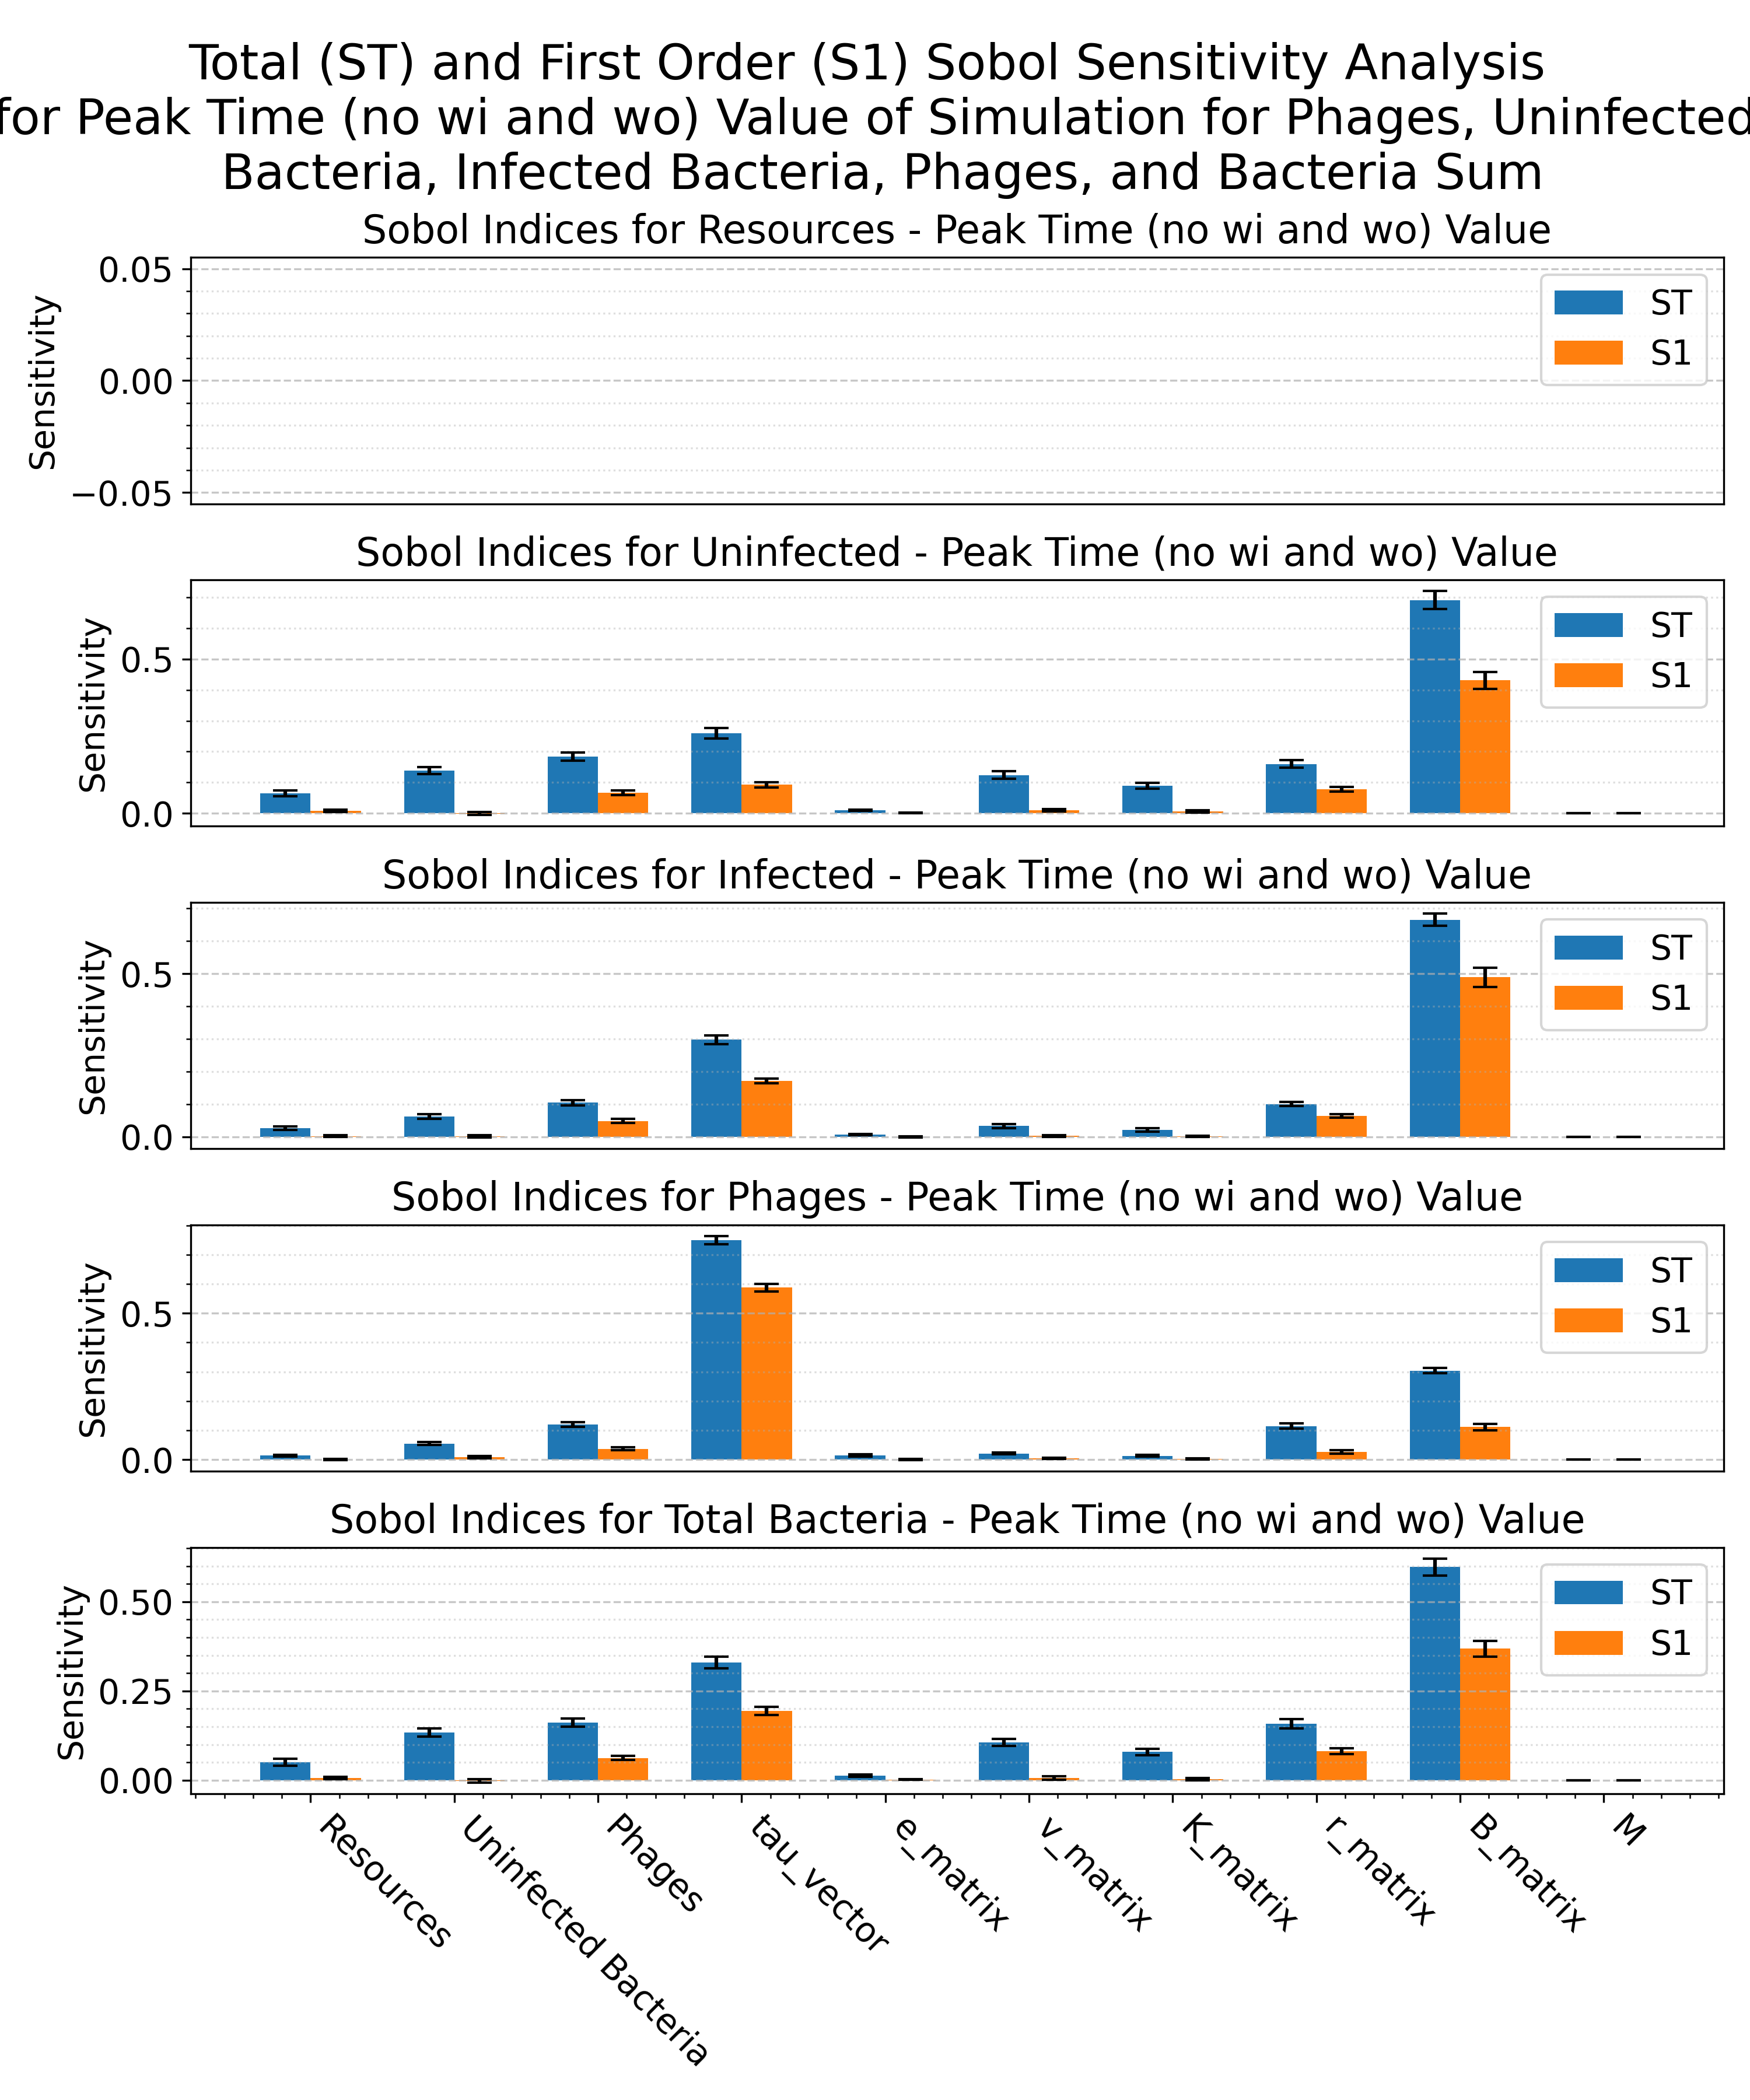
\includegraphics[width=\linewidth]{Plots/Created/SOBOL_analysis_1748084143_Peak_Time_(no_wi_and_wo).png}
        \caption{
            Time of peak value, no washin and washout. 
        }
        \label{fig:created:SOBOL_peak_time_no_wi_wo_extra}
    \end{subfigure}
    \caption{
        SOBOL analyses for the final, average, variance, peak, and peak time, without a washin and washout rate.
        The data was saved from the dashboard and plotted using Matplotlib. 
        The values used for this SOBOL test can be found in \Cref{tab:appendixE:SOBOL_analysis_values}, except washin and washout have been set to 0. 
    }
    \label{fig:created:SOBOL_no_wi_wo_extra}
\end{figure}